\documentclass{standalone}
\usepackage{tikz}
\usepackage{ctex,siunitx,ninecolors}
\setCJKmainfont{Noto Serif CJK SC}
\usepackage{tkz-euclide}
\usepackage{amsmath}
\usepackage{wasysym}
\usetikzlibrary{patterns, calc}
\usetikzlibrary {decorations.pathmorphing, decorations.pathreplacing, decorations.shapes}
\begin{document}
\small
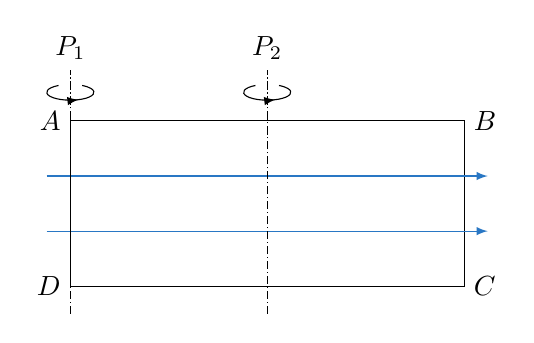
\begin{tikzpicture}[>=latex,scale=1.0]
  \draw(-2.5,-1.05)node[left]{$D$}rectangle(2.5,1.05)node[right]{$B$};
  \node at (-2.5,1.05)[left]{$A$};
  \node at (2.5,-1.05)[right]{$C$};
  \draw[->,azure5](-2.8,0.35)--(2.8,0.35);
  \draw[->,azure5](-2.8,-0.35)--(2.8,-0.35);
  \foreach \x[count =\i] in {-2.5,0}
    {
      \draw[thin,densely dashdotted](\x,-1.4)--(\x,1.7)node[above]{$P_\i$};
      \draw[postaction={decorate},decoration={markings,mark=at position 0.6 with {\arrow{>}}}](\x-0.15,1.5)arc(120:420:0.3 and 0.1);
    }
\end{tikzpicture}
\end{document}